\documentclass{article}
\usepackage[affil-it]{authblk}

\usepackage[final]{pdfpages}

\usepackage[utf8]{inputenc}
\usepackage{appendix}
\usepackage[numbers]{natbib}
\usepackage{pdfpages}
\usepackage{mathrsfs}
\usepackage{amsmath}
\usepackage{amsfonts}
\usepackage{amssymb}
\usepackage{setspace}
\usepackage{listings}
\usepackage[a4paper, total={6in, 8in}]{geometry}
\usepackage{xcolor}
\usepackage[separate-uncertainty = true,multi-part-units=single]{siunitx}
\usepackage{resizegather}

\definecolor{codegreen}{rgb}{0,0.6,0}
\definecolor{codegray}{rgb}{0.5,0.5,0.5}
\definecolor{codepurple}{rgb}{0.58,0,0.82}
\definecolor{backcolour}{rgb}{0.95,0.95,0.92}
 
\lstdefinestyle{mystyle}{
    backgroundcolor=\color{backcolour},   
    commentstyle=\color{codegreen},
    keywordstyle=\color{magenta},
    numberstyle=\tiny\color{codegray},
    stringstyle=\color{codepurple},
    basicstyle=\ttfamily\tiny,
    breakatwhitespace=false,         
    breaklines=true,                 
    captionpos=b,                    
    keepspaces=true,                 
    numbers=left,                    
    numbersep=3pt,                  
    showspaces=false,                
    showstringspaces=false,
    showtabs=false,                  
    tabsize=2
}
 
\lstset{style=mystyle}

\newcommand{\sig}[3]{($\num{#1} \pm #2$) \si{#3}}



\begin{document}


\begin{titlepage}
    \begin{center}
        \vspace*{1cm}
 
        \Large
        \textbf{An Application of Mach-Zehnder Interferometry to Measuring Refractive Index}\\
        
                \vspace{1cm}           

         \textbf{Carleton University}\\
        \vspace{1cm}
        \textbf{Department of Physics}\\
        \vspace{1cm}        
        \textbf{PHYS 4007 Lab 1 Report}\\
        
        \vspace{3cm}           
 
        \large
        \textbf{Author : Kenny(Kliti) Bala }\\
        \vspace{1cm}
        \textbf{Student Number : 100995430 }\\
        \vspace{1cm}
        \textbf{Section : Mon/Wed 2:30-5:30 PM}\\
        
        \vspace{3cm}

        \textbf{Date of Submission: \today}\\
        
        \vspace{3cm}
        
        \Large
        

        
        \vfill
    \end{center}
\end{titlepage}

\clearpage
\tableofcontents

\lstlistoflistings


\clearpage

\begin{abstract}
    A Mach-Zehnder Interferometer was assembled for the purpose of measuring the refractive
    index of water as a function of temperature. After assembly, a calibration was performed
    to determine the path length difference between the two interferometer beams as a function
    of the observed interference pattern, taken from a CCD camera. A sample of water was then
    heated, and placed in front of one of the interferometer paths. Recordings of fringe shifts
    as the sample cooled down were then made using an Si-based photodetector. The change in
    refractive index of the sample was then calculated from the observed fringe shift data.
    The calculated change in refractive index as a function of temperature was
    compared to an empirically derived model. The analysis of the collected data from the CCD camera
    led to an innacurate relation between expected and measured path length differences,
    indicating the setup was improperly aligned. In contrast, the comparison between measured
    changes in refractive index and predictions from a selected empirical model demonstrated
    an accurate calculation of refractive index from measured fringe shifts.
\end{abstract}

\section{ Introduction }\label{sec:introduction}
Optical interferometry is a ubiquitous technique in science and engineering which utilizes the
superposition of electromagnetic(EM) waves to extract measurements from the resulting interference patterns.
A Mach-Zehnder(MZ) Interferometer belongs to the category of amplitude-splitting optical interferometers.
This form of interferometry relies on the splitting of one primary wave into
two segments which can then interfere\cite[pg. 385]{hecht2002optics}.
This contrasts with wavefront-splitting interference such as a Young's double slit setup or a Fraunhofer diffraction setup, which produce interference through
recombination of secondary waves(waves generated from the diffraction of a primary wave through an aperture).
\par

In an MZ setup, a singular optical source is split into two separate paths, recombining at
a detector. The two separate paths will interfere completely constructively in the case where
the path lengths are equal. In cases of unequal path lengths, destructive interference will occur.
\par
The applications of the MZ interferometer has a multitude of applications in science and engineering.
A common application  low-cost, miniaturized sensors for parameters such as refractive index and
temperature\cite{Li:12}. In emerging fields, this technique also finds application in
quantum cryptography and computing\cite{Oliver1653}\cite{xavier2012employing}. In experimental
physics, the ability to observe single and double photon interference allows for investigation
of quantum physical phenomena\cite{Xavier:11}.
\par
By measuring the change in the observed interference pattern produced by a Mach-Zehnder interferometer,
we can measure the change in refractive index. This ability to measure refractive index changes can
be used to establish relationships between changes in a particular physical parameter, and 
refractive index which has numerous application in scientific measurement and also sensing.
\par
In this experiment, the change in refractive index as a function of temperature is investigated.
The temperature dependence of refractive index has been established for many compounds\cite{ametsoc_paper}.
Comparing already-established relationships to measurements from MZ interferometry will demonstrate
an interesting and relevant application of this technique in science and engineering.



\section{ Theory }\label{sec:theory}

\subsection{ Description Of The Optical System }\label{sec:description_of_the_optical_system}

A diagram of the MZ setup may be seen in Figure \ref{fig:mz_diagram_theory}. 
As can be seen, incident light from a laser is split into two separate paths by a beam splitter.
The two beams then get reflected off by two mirrors, recombining once more at another beam splitter.

\begin{figure}[h]
    \centering
    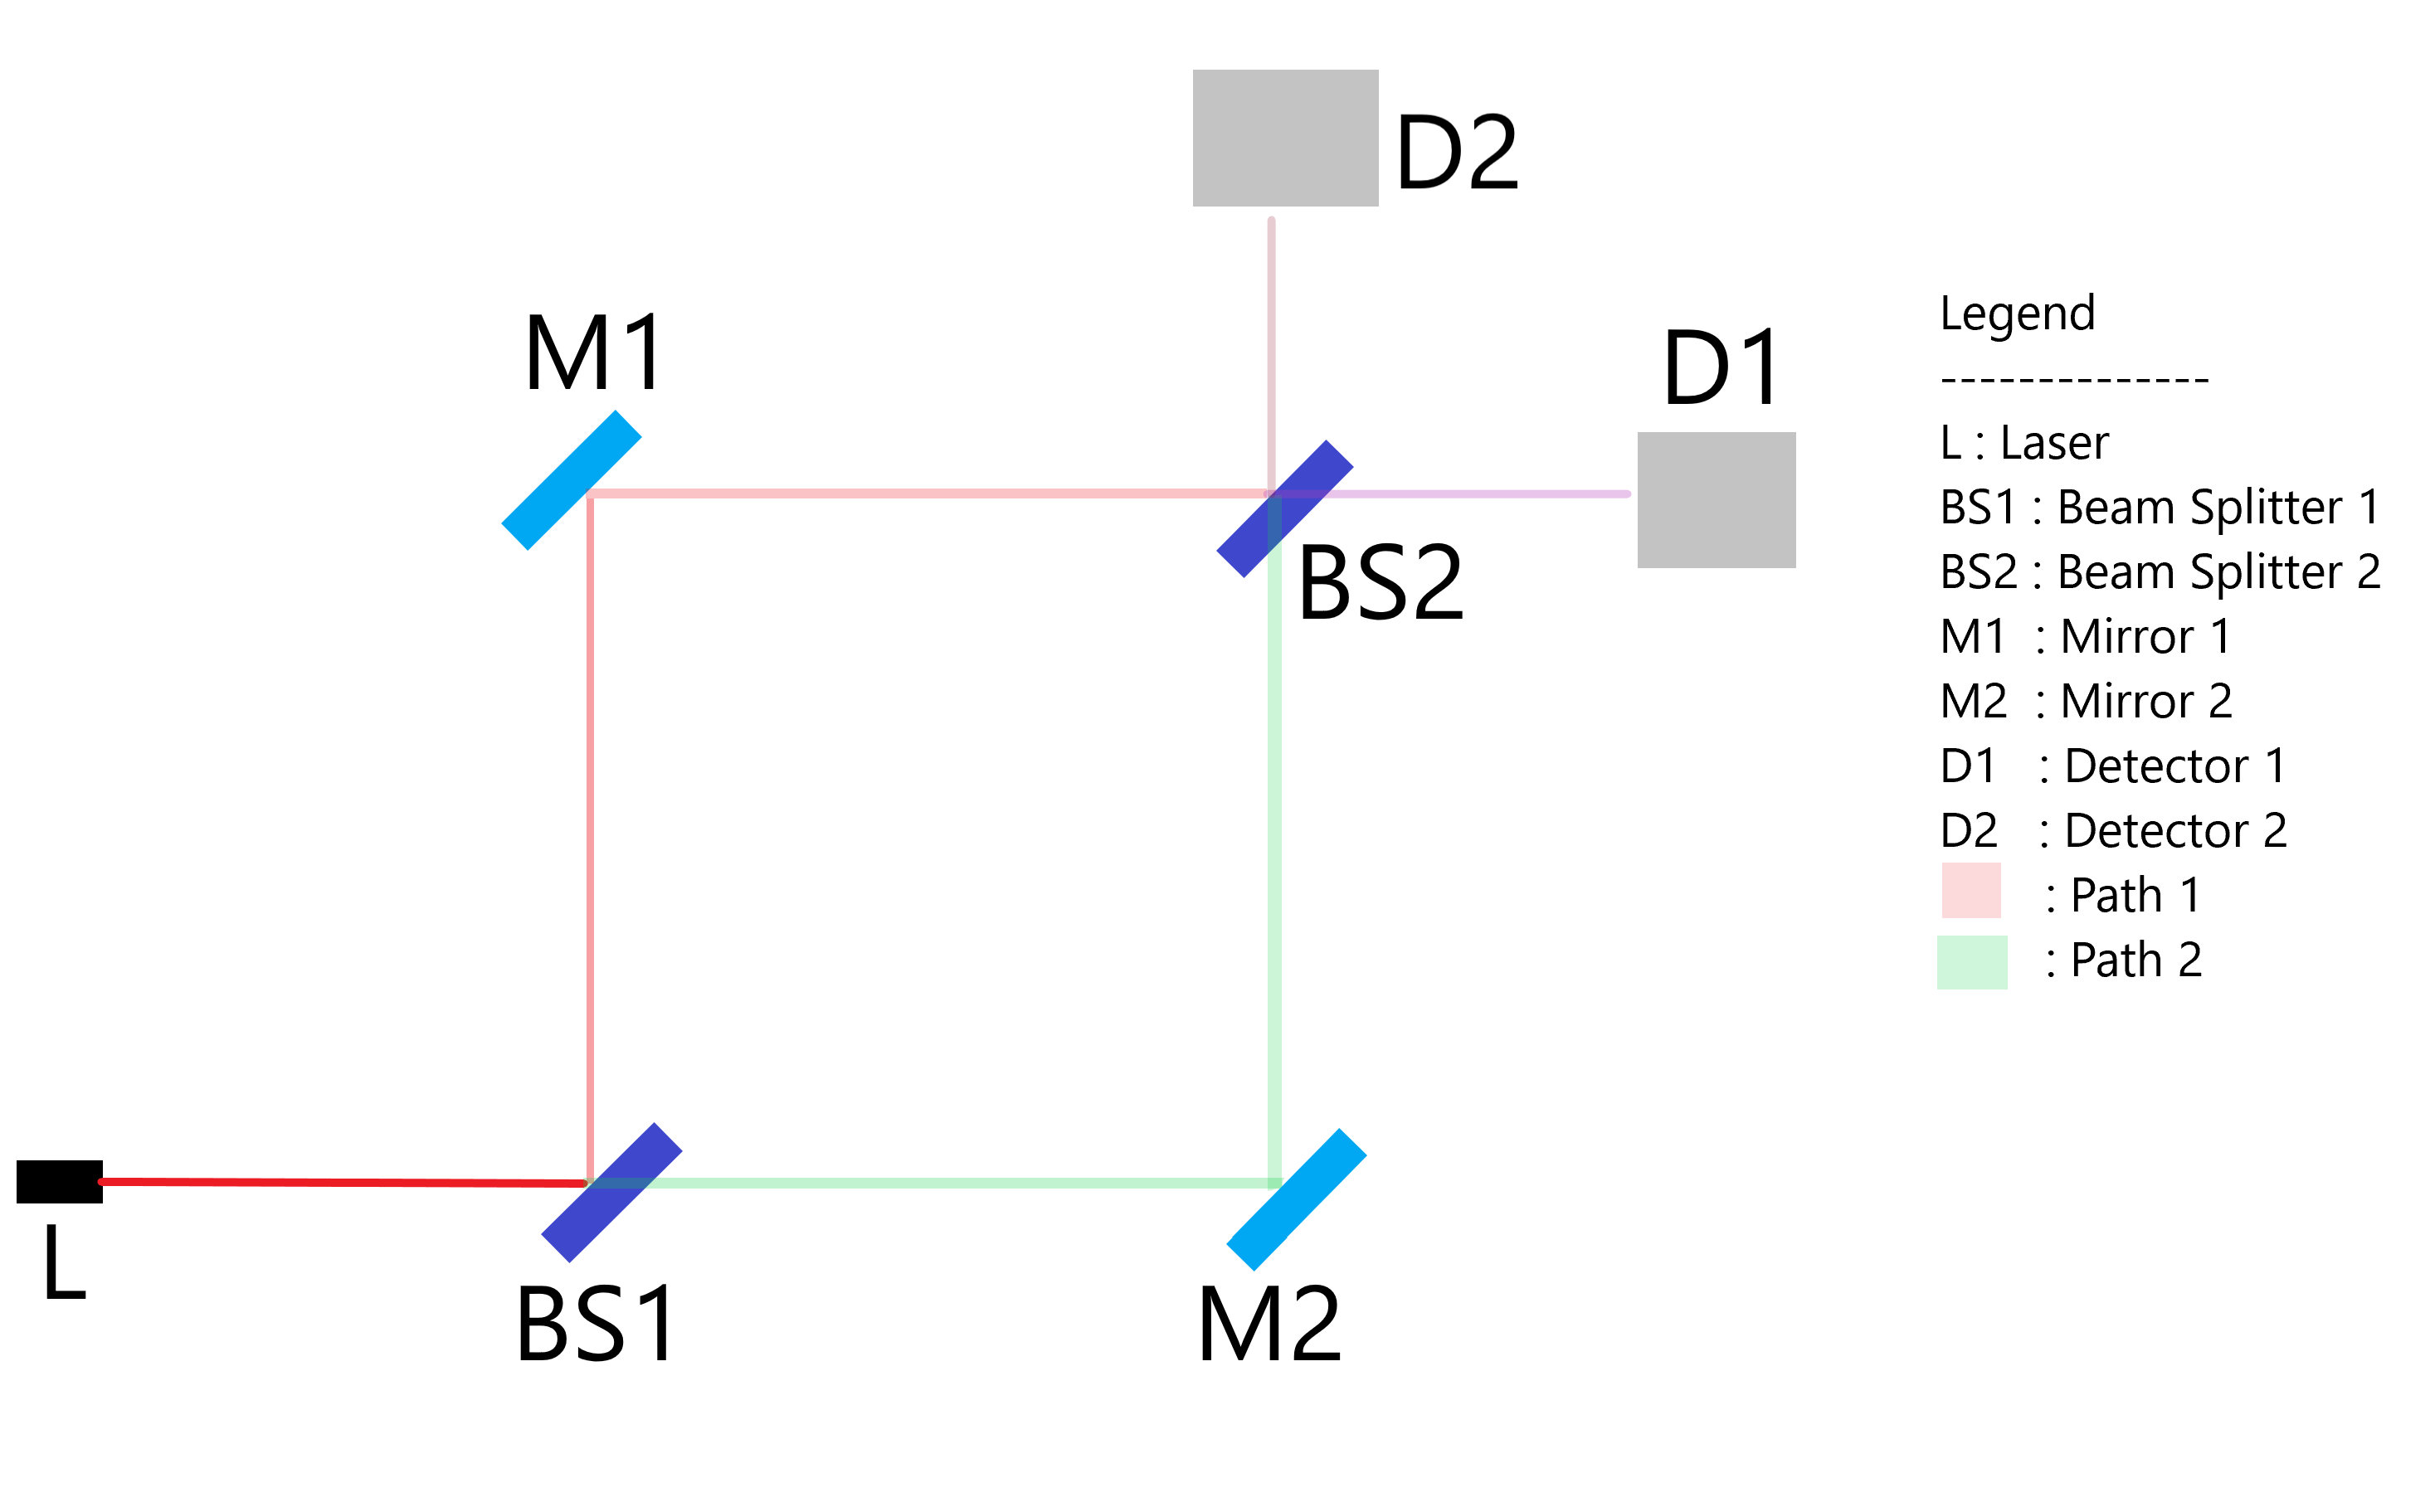
\includegraphics[width=4in]{images_theory/mz_diagram_theory.png}
    \caption{A Diagram of the MZ Optical System}
    \label{fig:mz_diagram_theory}
\end{figure}



\clearpage

\subsection{ Determining Phase Shift Between The Two Paths }\label{sec:determining_phase_shift_between_the_two_paths}
The phase difference between \textbf{Path 1} and \textbf{Path 2} may be determined by calculating the difference between path lengths\cite[pg. 48]{Zetie_2000}. Because only one detector
will be used in this experiment, we will only analyze the path of the two beams to \textbf{Detector 1}.
\par
Observing \textbf{Path 1},
we observe a reflection off the beam splitter \textbf{BS1} which shifts the phase by a factor of $\theta_{P1,BS1} = \pi$. We observe another phase shift at
mirror \textbf{M1} of $\theta_{P1,M1} = \pi$. We observe another phase shift through the beam splitter due to the transition from one material to another,
which equates to $\theta_{P1,BS2} = 2\pi{t}\lambda^{-1}$ where $t$ is the optical path length through the splitter, and $\lambda$ is the laser wavelength.
The final component of the phase for \textbf{Path 1} will be due to the actual real path length traversed, $\theta_{P1,l_1} = 2\pi{l_1}\lambda^{-1}$, where
$l_1$ is the real path length of \textbf{Path 1} not including the beam splitting component. This gives a final result of\cite[pg. 48]{Zetie_2000}:

\begin{equation}\label{eqn:phaseshiftp1}
    \theta_{P1} = \theta_{P1,BS1} + \theta_{P1,M1} + \theta_{P1,BS2} + \theta_{P1,l_1} = \pi + \pi + 2\pi{t}\lambda^{-1} + 2\pi{l_1}\lambda^{-1} = 2\pi + 2\pi\dfrac{l_1 + t}{\lambda}
\end{equation}

For \textbf{Path 2}, the analysis is essentially identical, but with the order reversed. The beam at \textbf{Path 2} first travels through \textbf{BS1} and incurs a phase shift of $\theta_{P2,BS1} = 2\pi{t}\lambda^{-1}$, incurs a $\pi$ shift at \textbf{M2}, and finally another $\pi$ phase shift at \textbf{BS2} where it reflects. Finally, it accumulates a path length phase shift
$\theta_{P2,l_2} = 2\pi{l_2}\lambda^{-1}$ from its own path length traversal $l_2$. This leads to the equation for net phase shift of \textbf{Path 2}\cite[pg. 48]{Zetie_2000}:

\begin{equation}\label{eqn:phaseshiftp2}
    \theta_{P2} = \theta_{P2,BS1} + \theta_{P2,M2} + \theta_{P2,BS2} + \theta_{P2,l_2} = 2\pi{t}\lambda^{-1} + \pi + \pi +2\pi{l_2}\lambda^{-1} = 2\pi + 2\pi\dfrac{l_2 + t}{\lambda}
\end{equation}

\par

We may now determine the final phase difference between the two paths, $\delta$\cite[pg. 48]{Zetie_2000}:

\begin{equation}\label{eqn:netphaseshift}
    \delta = \theta_{P1} - \theta_{P2} = 2\pi\dfrac{l_1 - l_2}{\lambda}.
\end{equation}

The key result of this analysis can be seen from Equation \ref{eqn:netphaseshift}. \textit{The net phase shift between paths depends on the path length difference between the two beams.}

\subsection{ Intensity Of The Interference Pattern As a Function of Path Length Difference }\label{sec:intensity_of_the_interference_pattern_as_a_function_of_path_length_difference}
We can also determine an expression for determining the path length difference as a function of interference pattern intensity.
This first begins with analyzing the net electric field, $\vec{E_t}$ produced by the superposition of the electric fields of two waves, $\vec{E_1}$ and $\vec{E_2}$ :
\begin{equation}
	\vec{E_t} = \vec{E_2} + \vec{E_1} = \vec{E_{01}}cos(kl_1 - \omega{t} + \phi_1) + \vec{E_{02}}cos(kl_2 - \omega{t} + \phi_2)
\end{equation}
Where $\vec{E_{01}},\vec{E_{02}}$  are the electric field magnitudes, $l_1,l_2$ are the path lengths travelled by each wave, $k = \frac{2\pi}{\lambda}$, and $\phi_1, \phi_2$ are the phases of the two waves Calculating the intensity $I_t$ produced by $\vec{E_t}$ , we get:

\begin{equation}
	I_t = \epsilon_o\cdot{c}\langle \vec{E_t} \cdot \vec{E_t} \rangle =  \epsilon_o\cdot{c}\langle (\vec{E_2} + \vec{E_1}) \cdot (\vec{E_2} + \vec{E_1}) \rangle = \epsilon_o\cdot{c} \bigg( \vec{E_1} \cdot \vec{E_1} + \vec{E_2} \cdot \vec{E_2} + \vec{E_1} \cdot \vec{E_2} \bigg) = I_1 + I_2 + I_{12}
\end{equation}where $I_{12}$ is the component of the intensity produced via wave interference. The $I_{12}$ term may be rewritten as:

\begin{equation}
	I_{12} = \vec{E_{01}}\vec{E_{02}}cos(kl_1 - \omega{t} + \phi_1)cos(kl_2 - \omega{t} + \phi_2)
\end{equation}Defining $\delta = k(l_2 - l_1) + (\phi_2 - \phi_1)$ and performing some trigonometric manipulation, we can write:

\begin{equation}
	I_{12} = \epsilon_o c \vec{E_{01}}\cdot\vec{E_{02}}cos(\delta)
\end{equation}
Since the MZ interferometer is of the amplitude-splitting variety, both waves will be \textit{mutually coherent}. This means that provided $(l_2 - l_1) < L$ where L is the coherence length of the light source, then $\phi_2(t) - \phi_1(t) = 0$. This gives $\delta = k(l_2 - l_1)$ and allows $I_t$ to be rewritten as:

\begin{equation}
	I_t = I_1 + I_2 + 2\sqrt{I_1I_2}cos(\delta)
\end{equation}

With further simplification from the above equation, we can write out the interference pattern as a function of path length\cite[pg. 388]{hecht2002optics}:

\begin{equation}
    \dfrac{I}{4I_o} = cos^2\bigg(\dfrac{\delta}{2}\bigg) =  \dfrac{1 + cos^2\bigg(2\dfrac{\delta}{2}\bigg)}{2} =  \dfrac{1 + cos(\delta)}{2}
\end{equation}

where $I$ is the intensity with a path difference of $\delta$, and $I_o$ is the intensity when $\delta = 0$. 

\subsection{ Observation of Fringes in the Interference Pattern }\label{sec:observation_of_fringes_in_the_interference_pattern}
The above explanation suffices for a non-extended source, such as a point-like beam with zero divergence. However, the laser being used does experience divergence in its beam. This means that $\delta$ varies as a function of the distance from the center of the imaging screen, and thus
depending on the viewing angle, the intensity measured is not uniform. Given the position on the imaging screen $x$, the intensity measured is:

\begin{equation}
	 \dfrac{I}{4I_o} =  \dfrac{1 + cos(\delta\cdot{x})}{2}
\end{equation}
Thus a larger path length difference increases fringe frequency, while a lower path length difference will decrease it. With perfect alignment,
the pattern is a purely bright fringe. With a path length difference that increases, the fringe frequency tends to infinity.
\subsection{ Dependence of Refractive Index on Temperature }\label{sec:dependence_of_refractive_index_on_temperature}
Paths of light obstructed by a material will experience a change in optical path length traversed, relative to an identical ray that is only traveling through vacuum.
The initial path length in a sample at in initial temperature $T_o$ with refractive index $n_o$ and thickness $d$ will be\cite[pg. 465]{flores2002}:

\begin{equation}
    l_{n_o} = \dfrac{n_o d}{\lambda}
\end{equation}

The refractive index if a material however, is not static. The value of this parameter will change based on a variety of physical conditions, one of them being the temperature of the material. The change to a new refractive index with a change in temperature $n$, will lead to a new optical path length through the material:

\begin{equation}
    l_{n} = \dfrac{n d}{\lambda}
\end{equation}

This can then be used to determine the phase difference between the two cases. This phase difference can also be translated to a change in the number of
fringes $\Delta{M}$ observed at the detector, as\cite[pg. 465]{flores2002}:

\begin{equation}
    \Delta{M} = \dfrac{(n - n_0)d}{\lambda}
\end{equation}

With an expression relating the shift in fringes as a function of refractive index,
we can now use simultaneous measurements of temperature and refractive index
to establish a relationship between the two quantities.

\subsection{ Comparing Results to an Empirical Model of Refractive Index of Water vs. Temperature }\label{sec:comparing_results_to_an_empirical_model_of_refractive_index_of_water_vs._temperature}
In order to compare the accuracy of results, it is important to compare results with published research on the topic of refractive index and its dependence on temperature. A simplified model for wavelength $\lambda$ and temperature $T$ was selected\cite{n_T_emp_model} which models $n(\lambda,T)$ using the Cauchy Formula as:

\begin{equation}
	 n(\lambda,T) =  A(T) + \dfrac{B(T)}{\lambda^2}  + \dfrac{C(T)}{\lambda^4}   + \dfrac{D(T)}{\lambda^6}
\end{equation}
where $A(T),B(T),C(T),D(T)$ are $3^{rd}$-order polynomial equations,
and $\lambda$ is a fixed value. Once data is collected for $\Delta{n} = n-n_o$ , we can
combine the predicted value of $n_o$ from $n(\lambda,T)$ with a running sum on $\Delta{n}$ to get $n_{exp}(T,\lambda)$, the experimentally calculated values of refractive index. We can then asses the accuracy of obtained results by applying a curve fit to $n_{exp}$ using the form of $n(\lambda,T)$ .

For the purpose of simplification, we can combine $A(T),B(T),C(T),D(T)$ together since they are all $3^{rd}$-order polynomials,
and $\lambda$ is a constant value. 


\section{ Experimental Setup }\label{sec:experimental_setup}

\subsection{ General Setup}\label{subsec:exp_setup_general_setup }\label{sec:general_setup}\label{subsec:exp_setup_general_setup}

The MZ interferometer apparatus was situated on top of a floating table, meant to keep all portions of the path that light goes through(mirrors, beam splitters, detectors) as free from vibrations as possible. Additionally, the floating table setup ensures that we can align the laser such that the emitted beam is parallel to the table setup at all points on the surface. This minimizes the path length difference variation due to vibrations, and also ensures we can get as close as possible to perfectly equal path lengths for both beams. Practically speaking however, perfect alignment and a perfectly vibration-free alignment was not possible with our setup.
\par
The light source for this setup was a 5mW HeNe laser with wavelength $\lambda$ = \sig{632.8}{10.53}{\nano \m} with an approximate coherence length of 30cm\cite{thorlabs.com_tutorials}\footnote{The spectral width of the laser produces an error on the final calculations of refractive index. This is discussed in Appendix \ref{app:wavelength_error_estimate}}. The laser was mounted on an adjustable stand which could rotate both the pitch and heading of the laser, in addition to adjusting the laser height. These functions were used for laser alignment.
\par
The mirrors were placed in mounts manufactured by Thor Labs. This allowed adjustment in both pitch and heading of the mirror, an important function for ensuring both mirrors in the setup were oriented at the same angle. These mounts were then placed on optical stands to keep them vertical, screwed into place on the floating table.
Additionally, optical posts were used for height adjustment.
\par
The beamsplitters were placed into mounts with pitch and heading adjustment as well, with post and post stands, all screwed into place onto the floating table.
\par
It is important to discuss the limitations of this setup in the context of alignment. The mounts and posts for both the mirrors and beamsplitters both experience tilt. This can be corrected by compensation(correcting the natural tilt of the mounts by adjusting pitch and heading, for example) but provides a limitation on the quality of the
alignment. However for the level of accuracy required in this experiment, these limitations can be compensated for.

\subsection{ Setup for Path Length Difference Measurements }\label{sec:setup_for_path_length_difference_measurements}

The setup for this part of the experiment was identical to configuration mentioned in Section \ref{subsec:exp_setup_general_setup}, but included
a CCD camera for imaging the interference pattern. Additionally, the 











\clearpage

\bibliographystyle{IEEEtran}
\bibliography{references}

\clearpage

\appendix


\section{ Example Calculations }\label{sec:example_calculations}

\subsection{ Temperature Conversion }\label{sec:temperature_conversion}

Conversion from a Type T thermocouple voltage $V$ to a temperature T is done by applying a set of coefficients to the recorded voltage. The conversion coefficients may be seen below.

\begin{equation}\label{eqn:temp_conversion}
    T = T_o +  \dfrac{ \Delta{V}( p_1 + \Delta{V}( p_2 + \Delta{V}(p_3 + p_4\Delta{V}))) }{ 1 + \Delta{V}(q_1 + \Delta{V}(q_2 + q_3\Delta{V})) }
\end{equation}

An example calculation using Equation \ref{eqn:temp_conversion} may be seen below(in MATLAB syntax).

\begin{lstlisting}[language=Matlab, caption=Example]

    % These are the coefficients for the voltage -> temperature conversion

    T0 = 1.3500000E+02;
    V0 = 5.9588600E+00;
    p1 = 2.0325591E+01;
    p2 = 3.3013079E+00;
    p3 = 1.2638462E-01;
    p4 = -8.2883695E-04;
    q1 = 1.7595577E-01;
    q2 = 7.9740521E-03;
    q3 = 0.0;
    
    V =  1.4094; % Recorded voltage in millivolts
    
    delta_v = V - V0;

    numerator = delta_v.*( p1 + delta_v.*( p2 + delta_v.*(p3 + p4.*delta_v)));
    denominator = 1 + delta_v.*(q1 + delta_v.*(q2 + q3.*delta_v));
    T = T0 + numerator./denominator;

    T =

   35.1559

\end{lstlisting}

\clearpage

\subsection{ Temperature Conversion Error Propagation }\label{sec:temperature_conversion_error_propagation}

First rewrite the expression as a polynomial.

\begin{equation}
	T = T_o + \frac{p_1\Delta{V} + p_2\Delta{V}^2 + p_3\Delta{V}^3 + p_4\Delta{V}^4}{ 1 + q_1\Delta{V} + q_2\Delta{V}^2}
\end{equation}

Taking the partial derivative by using the quotient rule:

\begin{gather}
	\frac{\partial{T}}{\partial{\Delta{V}}} = \frac{  (p_1 + 2p_2\Delta{V} + 3p_3\Delta{V}^2 + 4p_4\Delta{V}^3)( 1 + q_1\Delta{V} + q_2\Delta{V}^2) - (p_1\Delta{V} + p_2\Delta{V}^2 + p_3\Delta{V}^3 + p_4\Delta{V}^4)(q_1 + 2q_2\Delta{V})}{ (1 + q_1\Delta{V} + q_2\Delta{V}^2)^2}
\end{gather}

Since this only depends on one variable($\Delta{V}$) the error becomes:

\begin{equation}
	\sigma_T = \sqrt{\frac{\partial{T}}{\partial{\Delta{V}}}^2\sigma_V^2} = \frac{\partial{T}}{\partial{\Delta{V}}}\sigma_V
\end{equation}






\clearpage

\subsection{ Theoretical Calculation of Refractive Index }\label{sec:theoretical_calculation_of_refractive_index}

\begin{lstlisting}[language=Matlab, caption=Example]

 

lambda = 632.8; % The empirical equation takes in lambda in nanometers
T = 35; % Example temperature of 35 C

% Empirical model coefficients

A = [5.0233e-9 -1.8674e-6 -1.2325e-5 1.3208];
B = [6.9608e-5 -2.284e-2 -0.5179 5208.2413 ]/lambda^2;
C = [ 2.7729 -917.2319 -18341.336 -2.5551e8]/lambda^4;
D = [-1.2932e-7 3.6733e-5 1.7855e-3 9.3495]/lambda^6;

% Both lambda and A,B,C,D are constants.
%They are also all polynomials of equal order.
% Thus, we can add them all together.

empirical_model_coefficients = A + B + C + D;

empirical_model_coefficients = 

[5.214424e-10  -1.930158079e-7  -1.3732724725e-6   1.332212968308965]

% Use "polyval" to evaluate a polynomial with T as the variable and empirical_model_coefficients as the polynomial coefficients

n_theory = polyval(coefficients_empirical,T);

n_theory = 
       1.329591447705452


\end{lstlisting}

\clearpage

\subsection{ Error Propagation for Empirical Model Refractive Index }\label{sec:error_propagation_for_empirical_model_refractive_index}

The error propagation equation for the empirical model $n(T, \lambda)$ is:

\begin{equation}
    \sigma_{n(T,\lambda)} = \sqrt{ \bigg(\dfrac{\partial{n}}{\partial{T}}\bigg)^2(\sigma_T)^2 + \bigg(\dfrac{\partial{n}}{\partial{\lambda}}\bigg)^2(\sigma_\lambda)^2}
\end{equation}
Calculating $\dfrac{\partial{n}}{\partial{T}}$ :

\begin{equation}
	\dfrac{\partial{n}}{\partial{T}} = 
    \dfrac{\partial}{\partial{T}}\bigg[   A(T) + \dfrac{B(T)}{\lambda^2}  + \dfrac{C(T)}{\lambda^4}   + \dfrac{D(T)}{\lambda^6}\bigg] =
    \bigg[ B^{'} + \dfrac{C^{'}}{2}T + \dfrac{D^{'}}{3}T^2 \bigg]
\end{equation}
Calculating  $\dfrac{\partial{n}}{\partial{\lambda}}$  :

\begin{equation}
\dfrac{\partial{n}}{\partial{\lambda}} = 
    \dfrac{\partial}{\partial{\lambda}}\bigg[   A(T) + \dfrac{B(T)}{\lambda^2}  + \dfrac{C(T)}{\lambda^4}   + \dfrac{D(T)}{\lambda^6}\bigg] =
    \bigg[   \dfrac{-2B(T)}{\lambda^3}  + \dfrac{-4C(T)}{\lambda^5}   + \dfrac{-6D(T)}{\lambda^7}\bigg]
\end{equation}
\subsection{ Example Calculation of Change in Refractive Index }\label{sec:example_calculation_of_change_in_refractive_index}

Given $\lambda = 632nm, d = 5cm, \Delta{m} = 1$ , we can write:


\begin{equation}
	\Delta{n} =  n - n_o=\frac{\lambda\Delta{m}}{d} = \frac{632nm(1)}{5cm} = \num{1.264d-5}
\end{equation}



\clearpage

\subsection{ Error Estimation for HeNe Laser Wavelength}\label{app:wavelength_error_estimate }\label{sec:error_estimation_for_hene_laser_wavelength}\label{app:wavelength_error_estimate}
We can use the coherence length of approximately 30cm for an HeNe laser. Using this value and the expression for coherence length $L$:

\begin{equation}
	L = \frac{\lambda}{n\Delta\lambda} \rightarrow \Delta\lambda = \frac{\lambda}{nL} = \frac{632nm}{(1.0003)(30cm)} = 0.00000210603m = 21.06nm
\end{equation}Dividing this value by two, we can get an approximate $\sigma_\lambda = \pm 10.53nm$ 




\subsection{ Error Propagation for Experimentally Derived Refractive Index }\label{sec:error_propagation_for_experimentally_derived_refractive_index}

\begin{equation}
	1 = \frac{\Delta{n}\cdot d}{\lambda} \rightarrow \Delta{n} = \frac{\lambda}{d}
\end{equation}The error propagation equation is:

\begin{equation}
	\sigma_{\Delta{n}} = \sqrt{ \bigg(  \frac{\partial\Delta{n}}{\partial\lambda} \bigg)^2\sigma_\lambda^2 + \bigg( \frac{\partial\Delta{n}}{\partial{d}}  \bigg)^2\sigma_d^2} = \sqrt{ \bigg(  \frac{1}{d} \bigg)^2\sigma_\lambda^2 + \bigg( \frac{-\lambda}{d^2}  \bigg)^2\sigma_d^2}
    = \sqrt{ \bigg(  \frac{1}{5cm} \bigg)^2(10.53nm)^2 + \bigg( \frac{-632nm}{5cm^2}  \bigg)^2(0.05cm)^2} = \num{2.4562d-7}
\end{equation}
However this is the expression on a fringe-to-fringe basis. For calculating $n$ where $\Delta{m} > 1$, we need to apply this error propagation recursively.
For $n = n_o + \Delta{n} + \Delta{n}$ or in the case where you observe two fringe shifts, the error would be:

\begin{equation}
	\sigma_{n,2} = \sqrt{\sigma_{\Delta{n}}^2 + \sigma_{\Delta{n}}^2} = \sqrt{2}\sigma_{\Delta{n}}
\end{equation}Then for an fringes:

\begin{equation}
	\sigma_{n,3} = \sqrt{\sigma_{\Delta{n,2}}^2 + \sigma_{\Delta{n}}^2} =\sqrt{(\sqrt{2}\sigma_{\Delta{n}})^2 + \sigma_{\Delta{n}}^2} = \sqrt{3}\sigma_{\Delta{n}}
\end{equation}For $N$ fringe transitions, the error is then:

\begin{equation}
  \sigma_{n,N} = \sqrt{N}\sigma_{\Delta{n}}
\end{equation}





\clearpage

\section{ Part 1 Analysis }\label{sec:part_1_analysis}

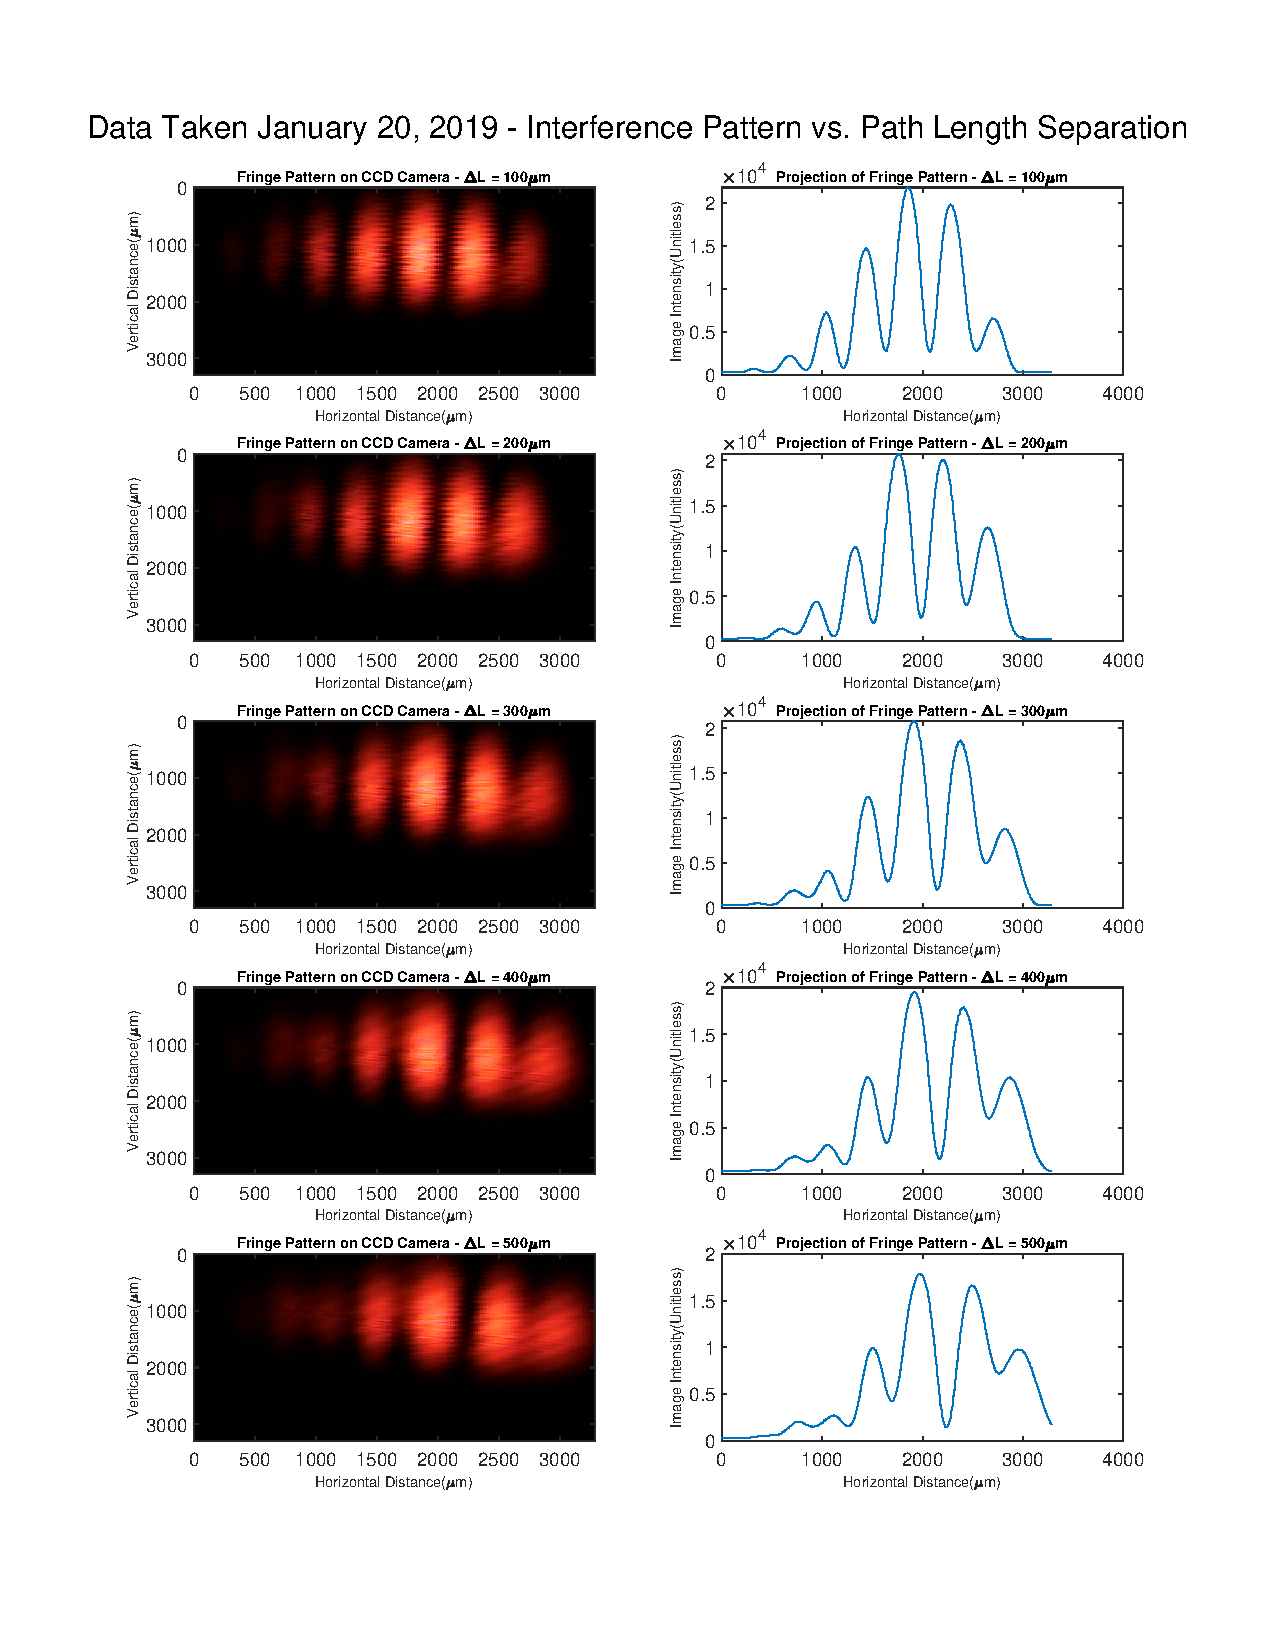
\includepdf[pages=-]{images_analysis/interference_pattern_jan_20_data.pdf}

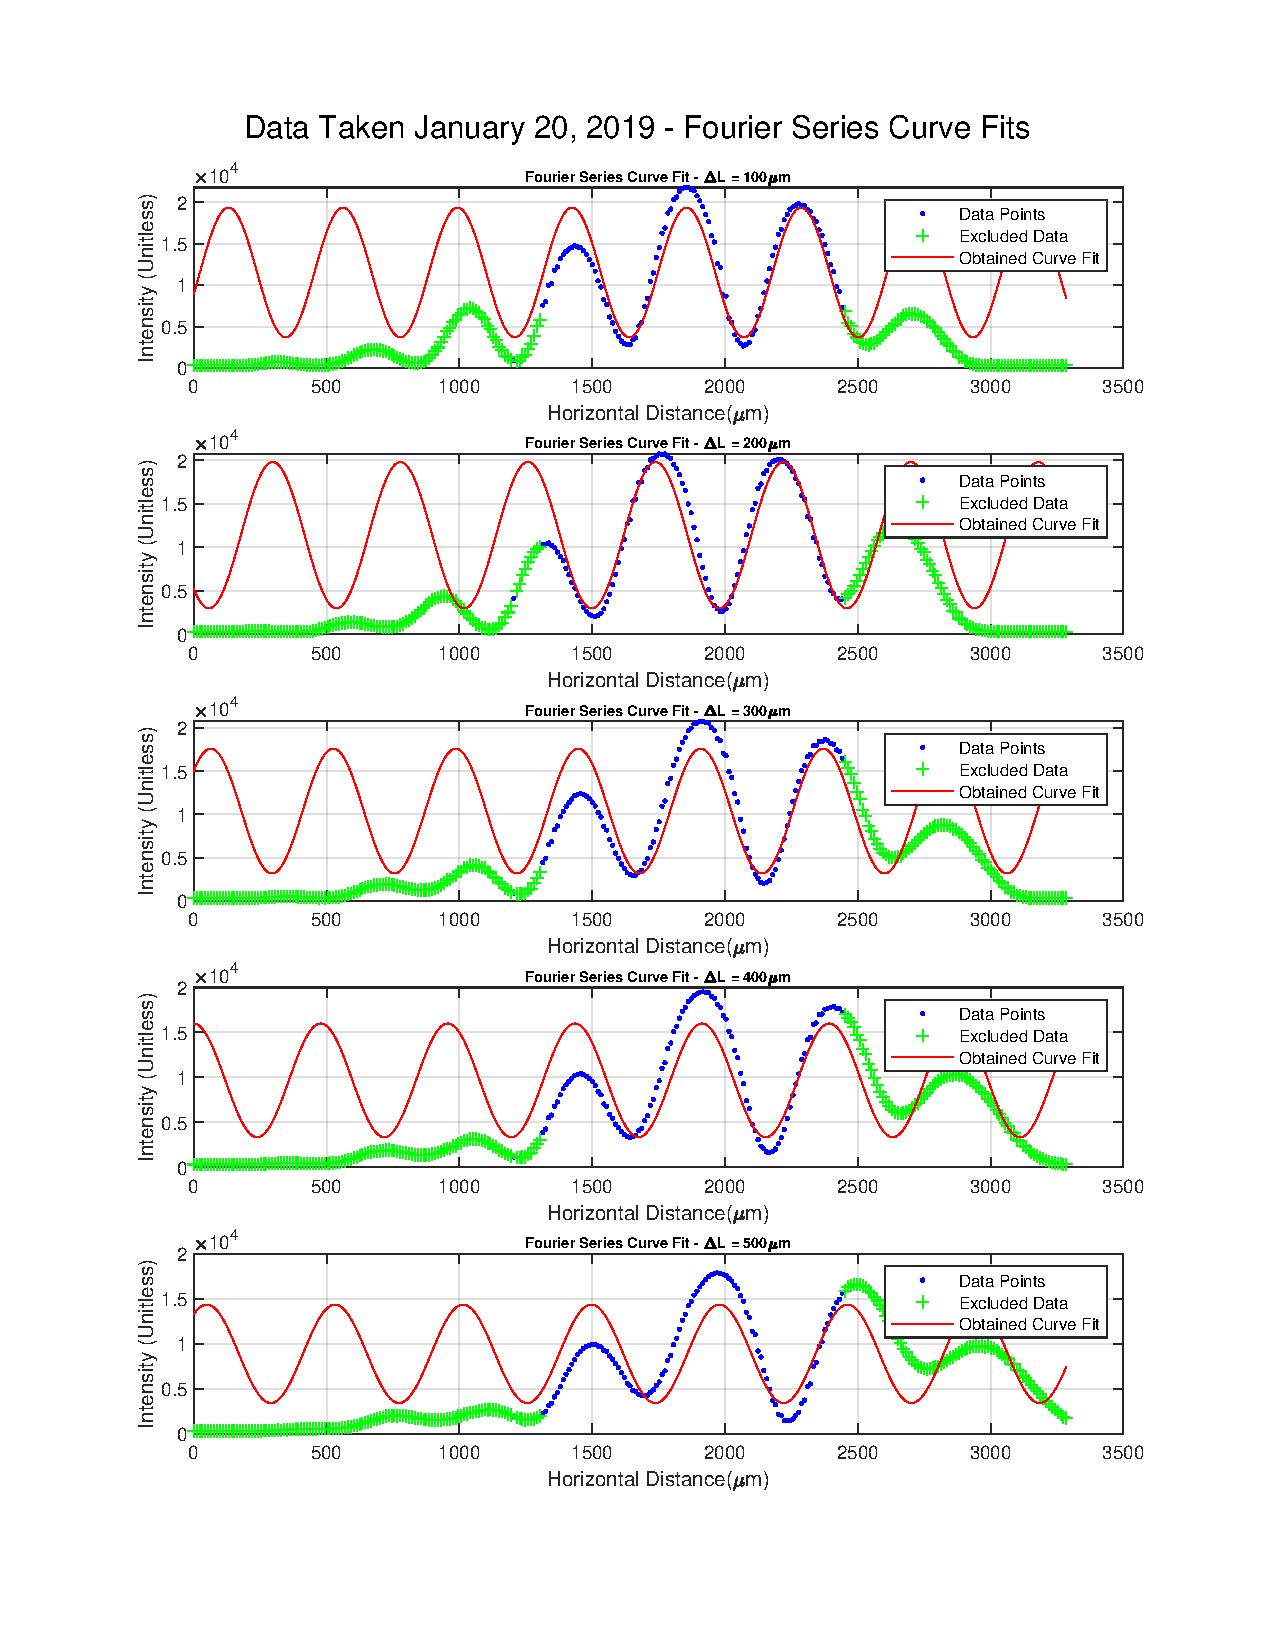
\includepdf[pages=-]{images_analysis/curve_fits_jan_20_data.pdf}

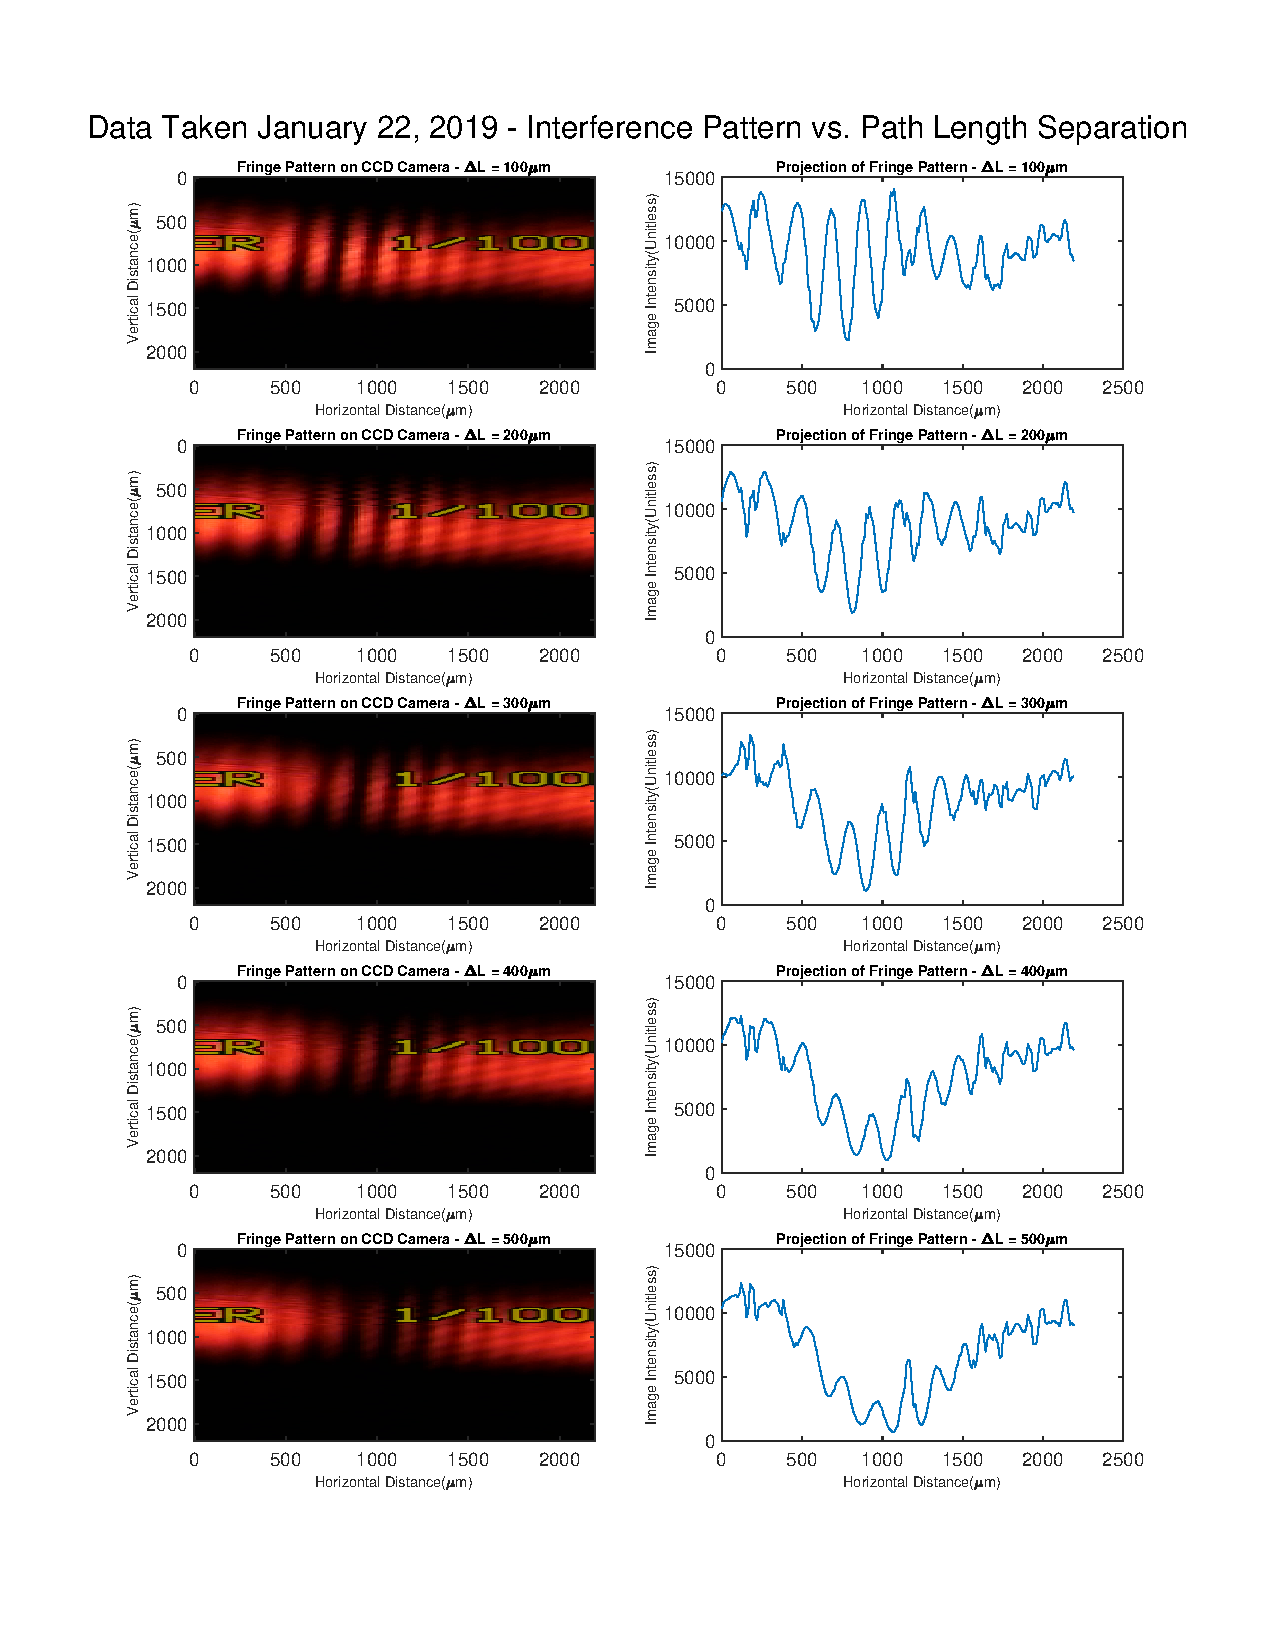
\includepdf[pages=-]{images_analysis/interference_pattern_jan_22_data.pdf}

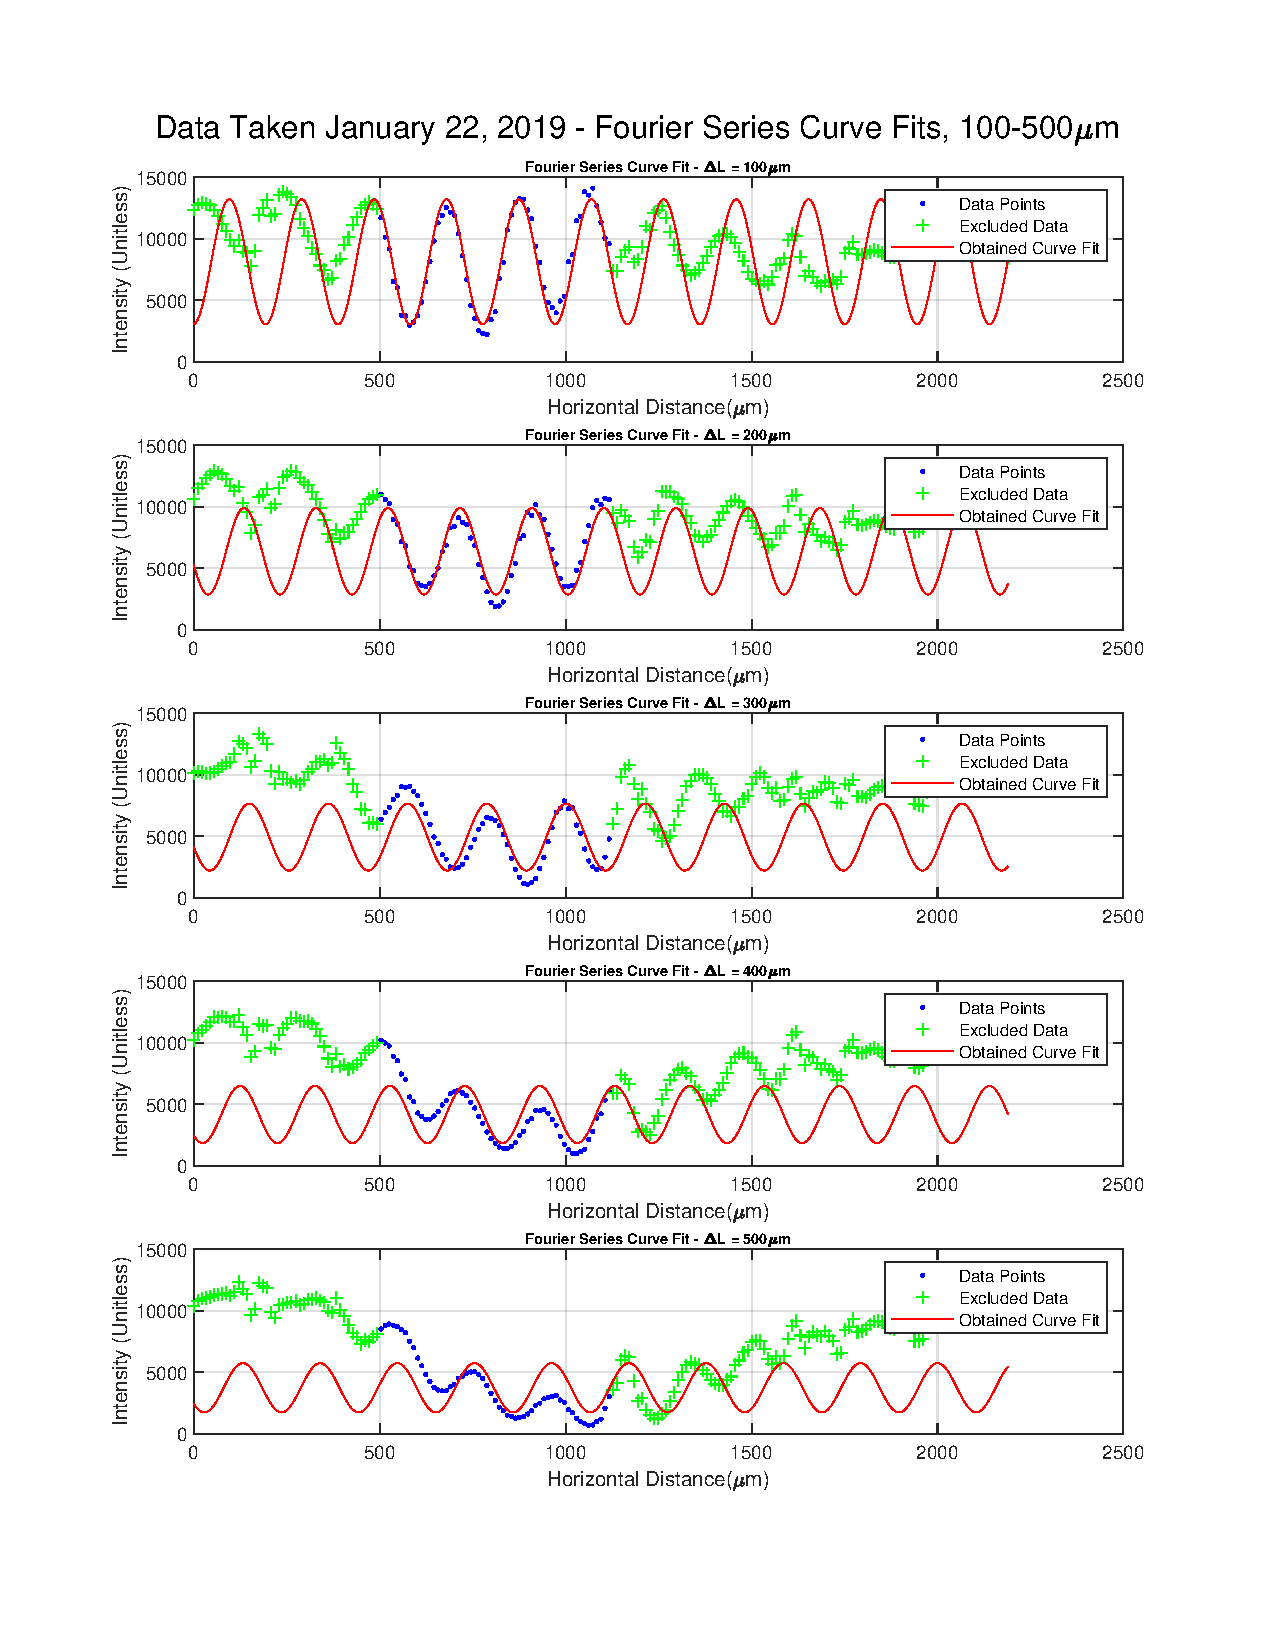
\includepdf[pages=-]{images_analysis/curve_fits_jan_22_data.pdf}

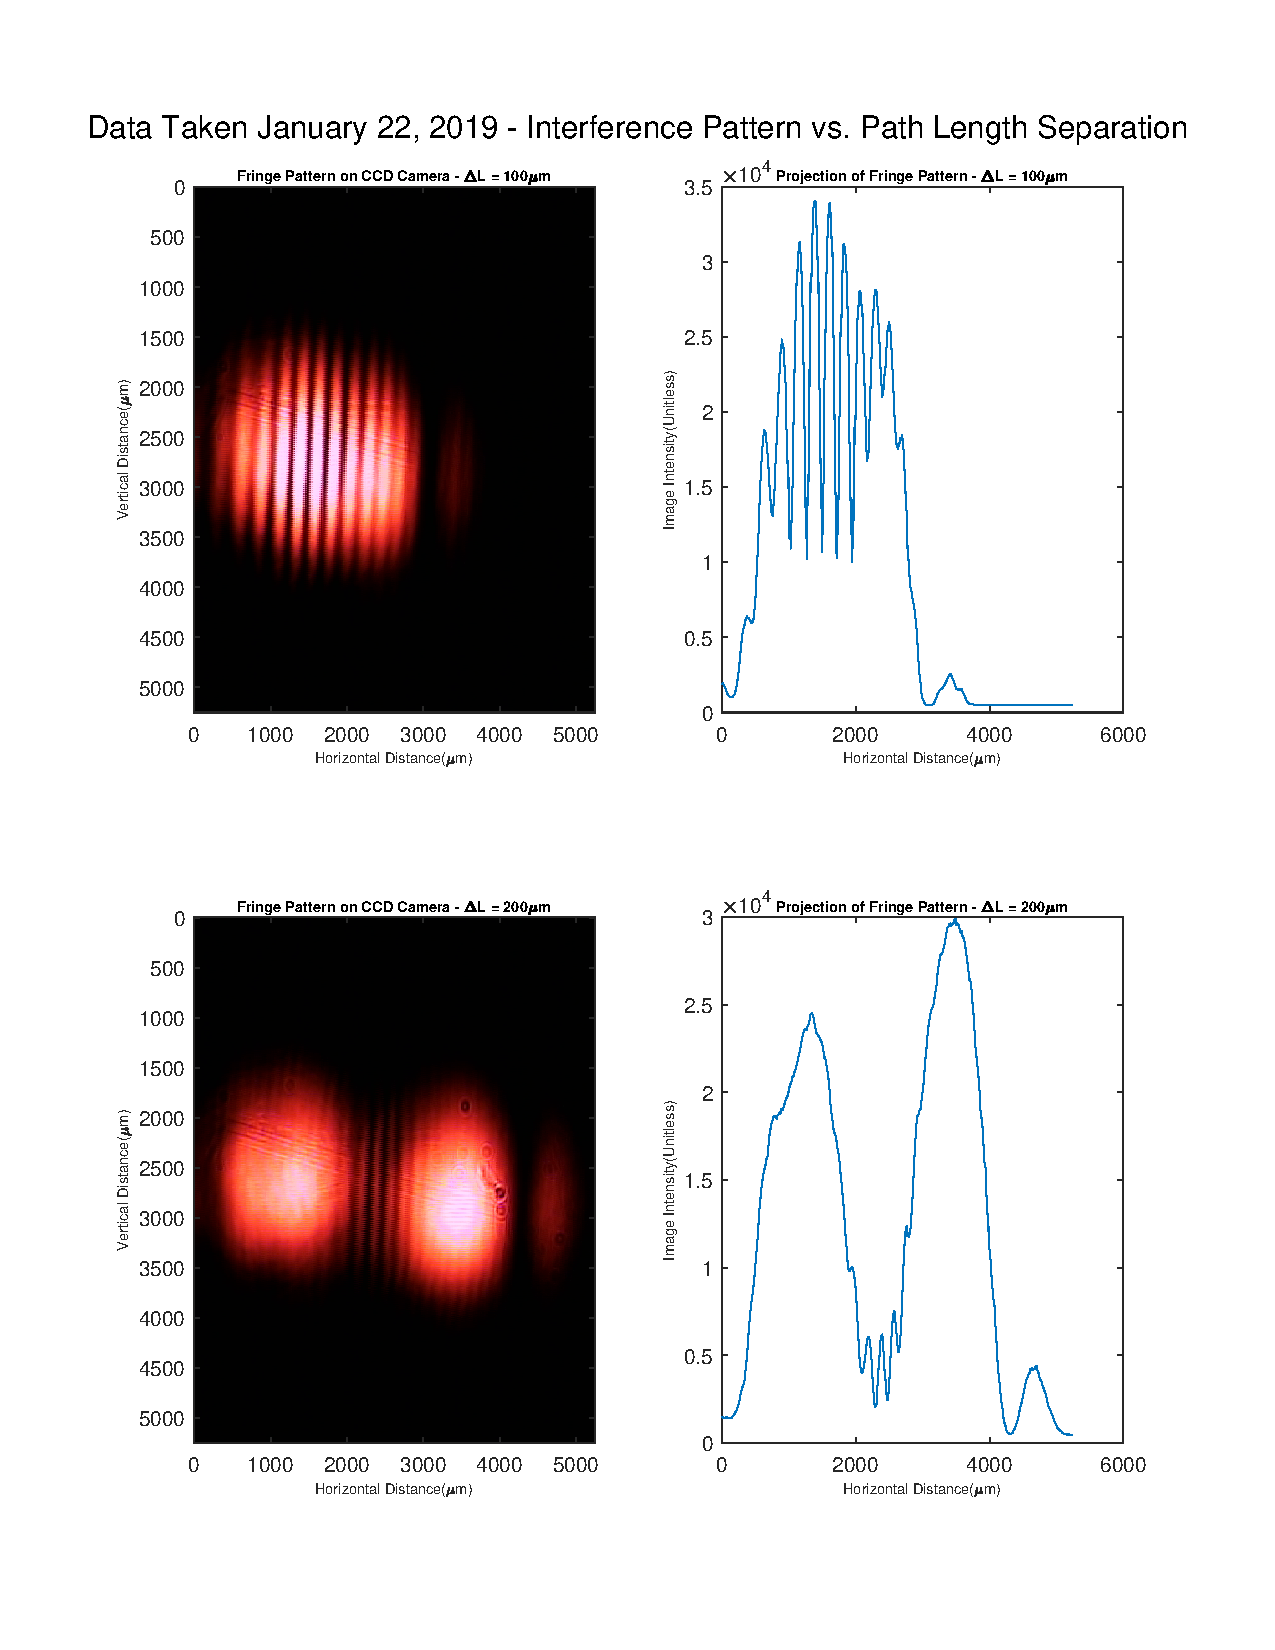
\includepdf[pages=-]{images_analysis/interference_pattern_jan_22_data_final_inc.pdf}

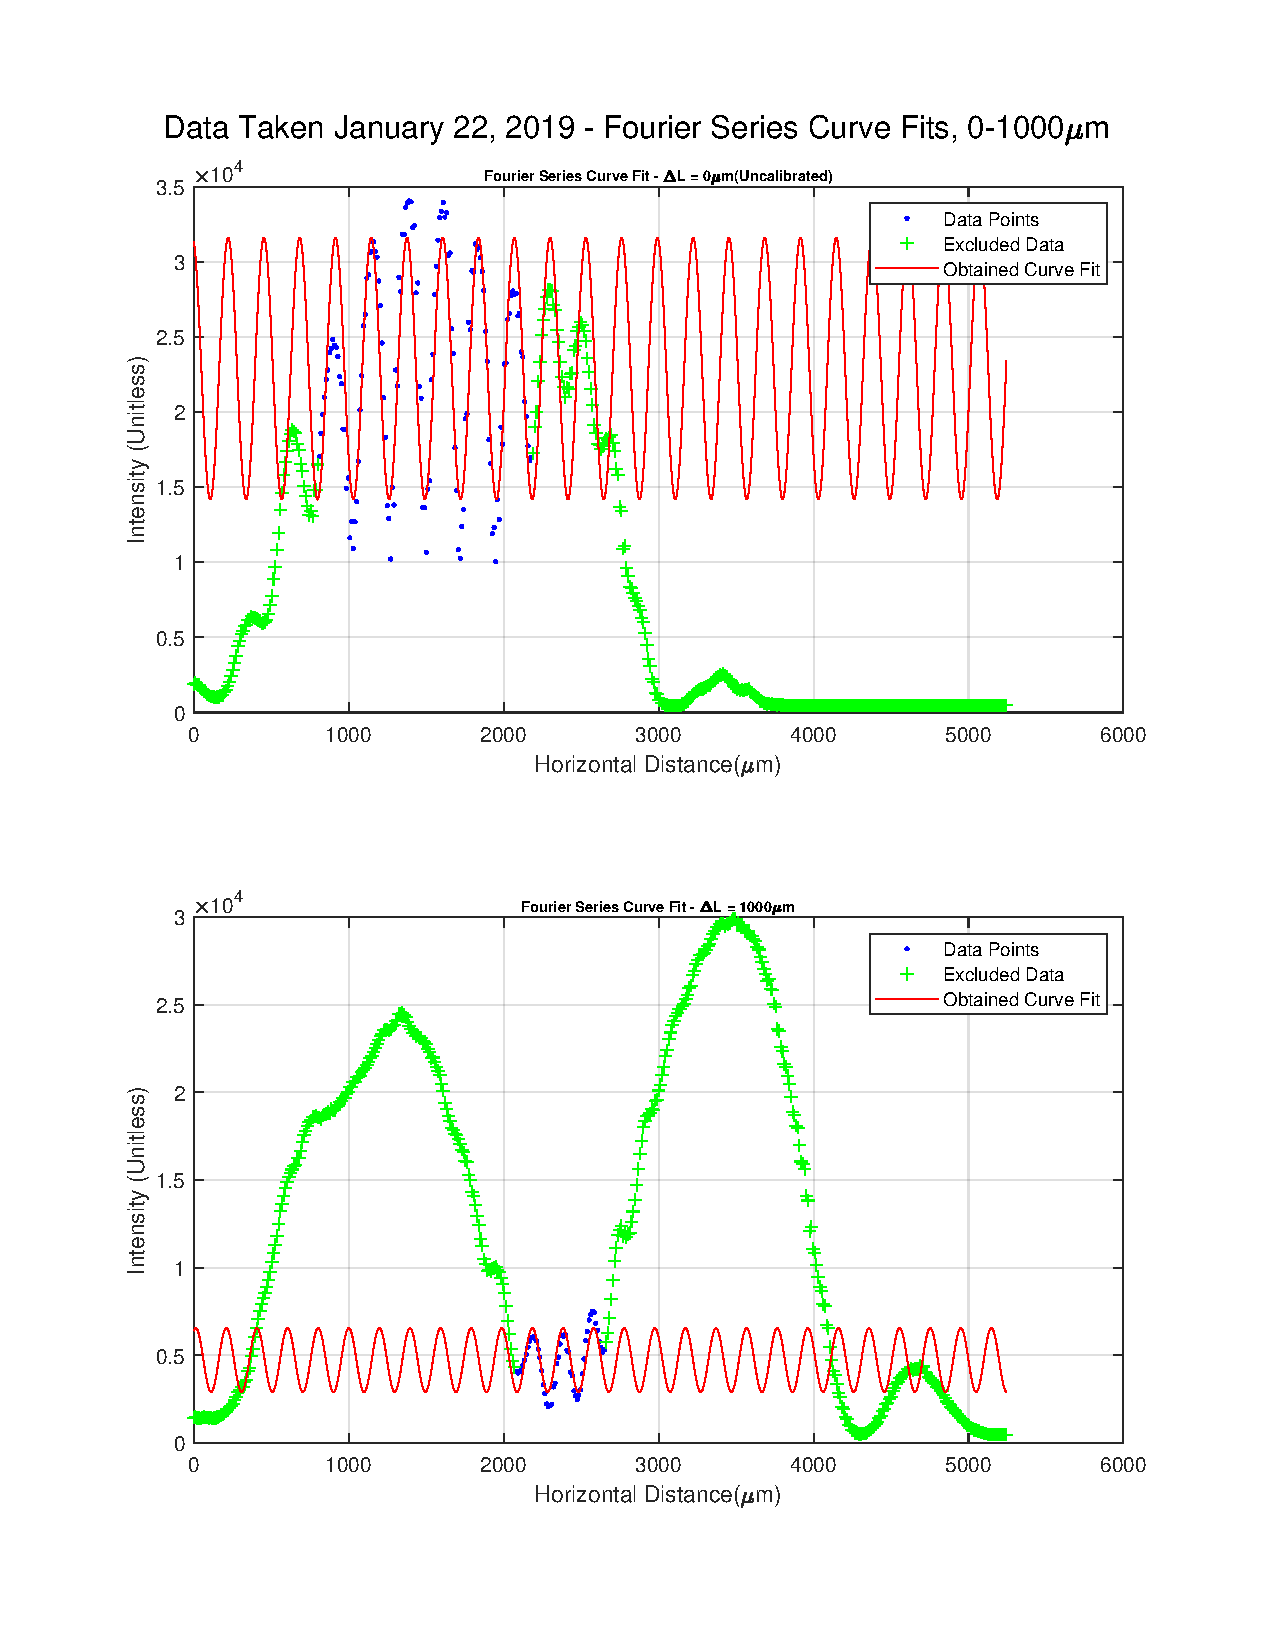
\includepdf[pages=-]{images_analysis/curve_fits_jan_22_data_final_inc.pdf}

\end{document}
